\documentclass[a4paper,11pt]{report}

\usepackage{amsmath,amssymb,amsthm}
\usepackage{fullpage}
\usepackage{graphicx}

\usepackage{bussproofs}
\usepackage{mathpartir}
\usepackage{prooftrees}
\usepackage{color}
\usepackage{rotating}



\usepackage{tikz}
\usetikzlibrary{automata,positioning}
\usetikzlibrary{fit}

\newcommand*\circled[1]{\tikz[baseline=(char.base)]{
    \node[shape=circle,draw,inner sep=2pt] (char) {#1};}}

\makeatletter
\pgfmathdeclarefunction{alpha}{1}{%
  \pgfmathint@{#1}%
  \edef\pgfmathresult{\pgffor@alpha{\pgfmathresult}}%
}

\newcommand*{\until}{U}
\newcommand*{\disj}{\ ,\ }
\newcommand*{\A}{\square}  % Always
\newcommand*{\D}{\diamondsuit} % eventually

\newcommand*{\Pq}{(\top,\bot)}
\newcommand*{\pQ}{(\bot,\top)}
\newcommand*{\PQ}{(\top,\top)}
\newcommand*{\pq}{(\bot,\bot)}


% tikz
\usepackage{tikz}
\usetikzlibrary{snakes}


\author{Sylvain Julmy}
\date{\today}

\setlength{\parindent}{0pt}
\setlength{\parskip}{2.5pt}

\newtheorem*{thm}{Theorem}

\begin{document}

\begin{center}
  \Large{
    Automata on Infinite Structure\\
    Fall 2018
  }
  
  \noindent\makebox[\linewidth]{\rule{\linewidth}{0.4pt}}
  Exercice Sheet 11

  \vspace*{1cm}

  Author : Sylvain Julmy
  \noindent\makebox[\linewidth]{\rule{\linewidth}{0.4pt}}

  \begin{flushleft}
    Professor : Ultes-Nitsche Ulrich
    
    Assistant : Stammet Christophe
  \end{flushleft}

  \noindent\makebox[\linewidth]{\rule{\textwidth}{1pt}}
\end{center}

\section*{Exercise 1}

\begin{align*}
  & \exists x. (x \in Q_a \wedge x + 1 \in Q_b ) = \\
  & \exists x. (x \in X_0 \wedge \neg (x + 1 \in X_0) ) = \\
  & \exists X_1.( sing(X_1) \wedge X_1 \subseteq X_0 \wedge
    \exists X_2.( sing(X_2) \wedge succ(X_1,X_2) \wedge \neg (X_2 \subseteq X_0) ) ) = \\
  &  \exists X_1.\exists X_2.(X_1 \subseteq X_0 \wedge \neg(X_2 \subseteq X_0) \wedge succ(X_1,X_2))
\end{align*}


\subsection*{Automata for $X_1 \subseteq X_0$}

\begin{center}
  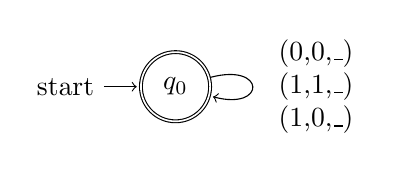
\begin{tikzpicture}[shorten >=1pt,node distance=2cm,on grid,auto]
    \tikzset{rounded/.style={draw,rectangle,rounded corners}}
    \node[state,accepting,initial] (q0) {$q_0$};
    \path[->]
    (q0)
    edge [loop right] node [] {$\begin{tabular}{c}(0,0,\_)\\(1,1,\_)\\(1,0,\_)\end{tabular}$} ()
    ;
  \end{tikzpicture}
\end{center}

\subsection*{Automata for $\neg(X_2 \subseteq X_0)$}

\begin{center}
  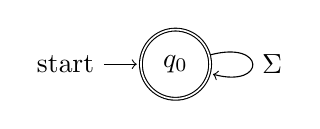
\begin{tikzpicture}[shorten >=1pt,node distance=2cm,on grid,auto]
    \tikzset{rounded/.style={draw,rectangle,rounded corners}}
    \node[state,accepting,initial] (q0) {$q_0$};
    \path[->]
    (q0)
    edge [loop right] node [] {$\Sigma$} ()
    ;
  \end{tikzpicture}
\end{center}

\subsection*{Automata for $succ(X_1,X_2)$}

\begin{center}
  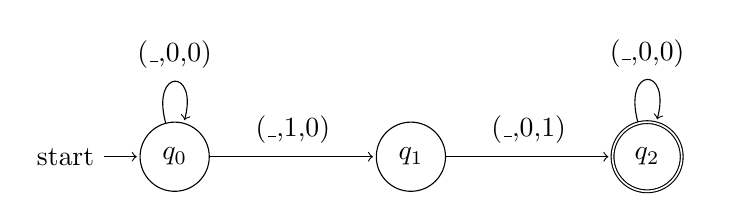
\begin{tikzpicture}[shorten >=1pt,node distance=3cm,on grid,auto]
    \tikzset{rounded/.style={draw,rectangle,rounded corners}}
    \node[state,initial] (q0) {$q_0$};
    \node[state] (q1) [right = of q0] {$q_1$};
    \node[state,accepting] (q2) [right = of q1] {$q_2$};
    \path[->]
    (q0)
    edge [loop above] node [above] {$\begin{tabular}{c}(\_,0,0)\end{tabular}$} ()
    edge [] node [] {$\begin{tabular}{c}(\_,1,0)\end{tabular}$} (q1)
    (q1)
    edge [] node [] {$\begin{tabular}{c}(\_,0,1)\end{tabular}$} (q2)
    (q2)
    edge [loop above] node [above] {$\begin{tabular}{c}(\_,0,0)\end{tabular}$} ()
    ;
  \end{tikzpicture}
\end{center}

\subsection*{Intersection}

\begin{center}
  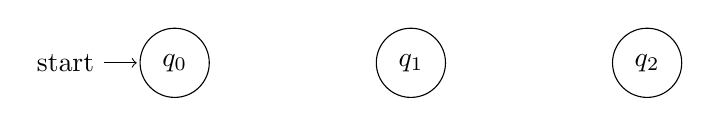
\begin{tikzpicture}[shorten >=1pt,node distance=3cm,on grid,auto]
    \tikzset{rounded/.style={draw,rectangle,rounded corners}}
    \node[state,initial] (q0) {$q_0$};
    \node[state] (q1) [right = of q0] {$q_1$};
    \node[state] (q2) [right = of q1] {$q_2$};
    \path[->]
    ;
  \end{tikzpicture}
\end{center}

\end{document}